\section{Electrical reproduction of sound}

\bi
\i A basic understanding of electricity and magnetism is 
needed to describe the functioning of musical recording 
and reproduction equipment.

\i Here, we briefly describe electrical circuits (voltage, current,
resistance, power, $\cdots$) and also Faraday's law of induction, 
which underlies the operation of microphones and loudspeakers.

\ei

%%%%%%%%%%%%%%%%%%%%%%%%%%%%%%%%%%%%%%%%%%%%%%%%%%%%%%%%%%%
\subsection{Basic electricity}

%
\begin{figure}[htbp]
\begin{center}
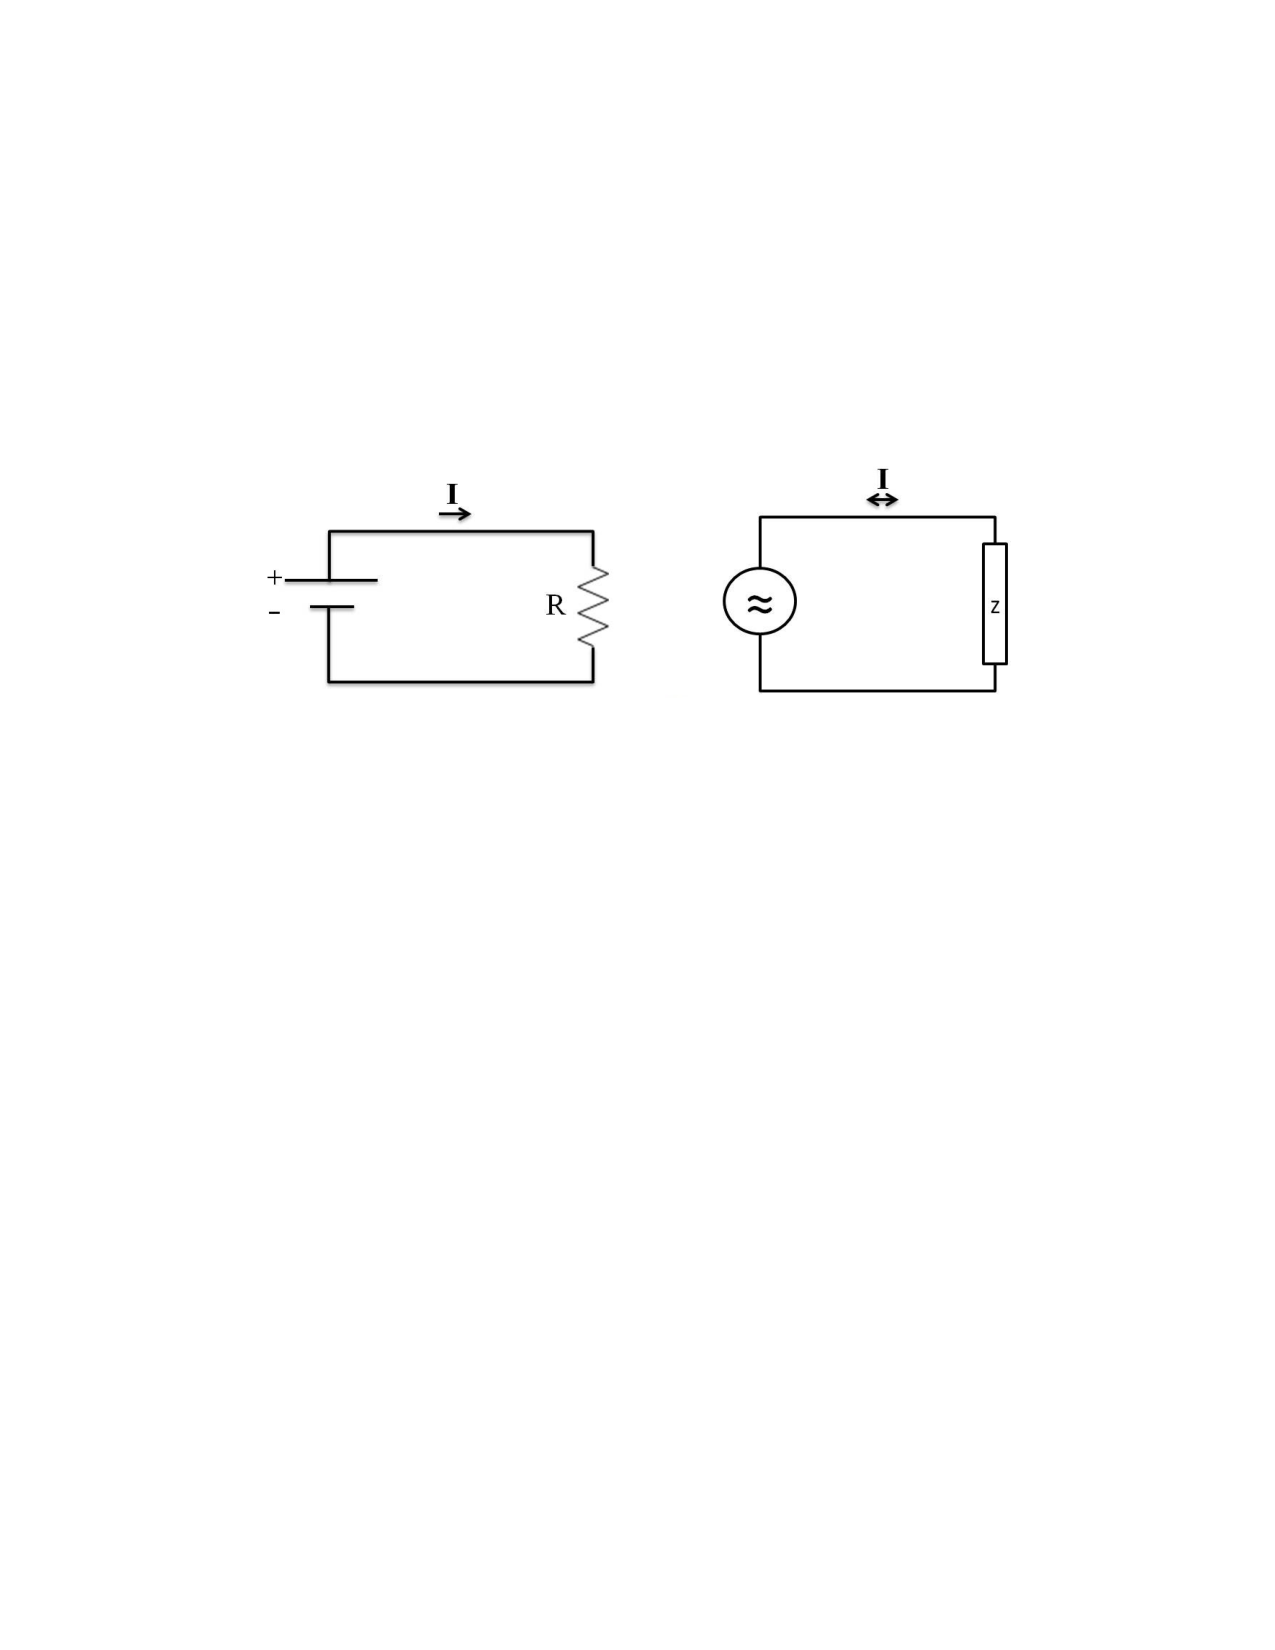
\includegraphics[width=0.7\textwidth]{circuits_DC_AC}
\caption{Left: Direct current (DC) circuit, consisting
of a voltage source and load having resistance $R$.
Right: Alternating current (AC) circuit, consisting of
a voltage sources and load having impedance $Z$.
For a DC circuit, the current flows in only one direction.
For an AC circuit, the current alternately flows clockwise and
counterclockwise.
(Figures from ``PHYS 1406: Physics of Sound \& Music" 
Course Guide by Prof.~Borst.)}
\label{f:circuits_DC_AC}
\end{center}
\end{figure}
%
%%%%%%%%%%%%%%%%%%%%%%%%%%%%%%%%%%%%%%%%%%%%%%%%%%%%%%%%%%%
\subsection{Faraday's law}

%
\begin{figure}[htbp]
\begin{center}
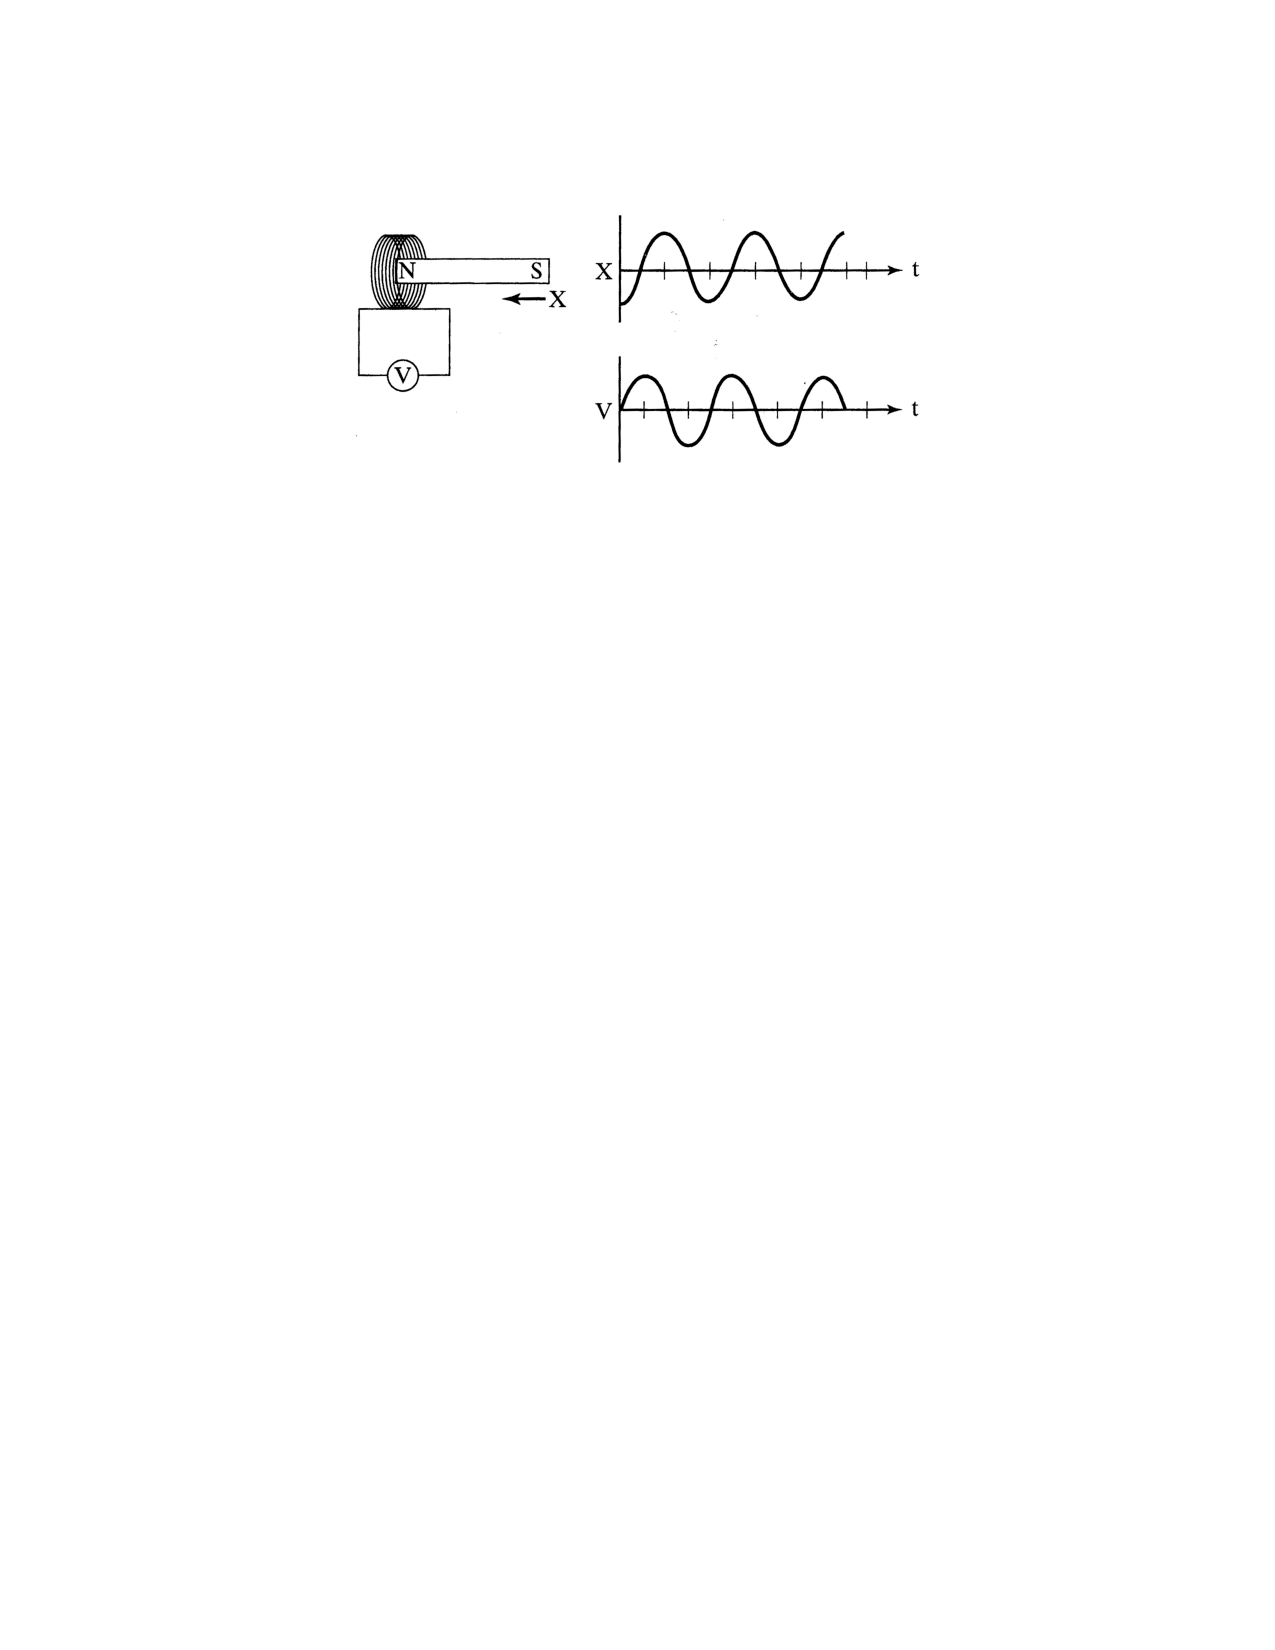
\includegraphics[width=0.6\textwidth]{faraday}
\caption{Illustration of Faraday's law.
As a magnetic moves back and forth ($X$ vs $t$) in the vicinty 
of a coil of wire, an alternating voltage ($V$ vs $t$) is induced
in the coil.
(Figure from ``Physics of Sound," by Berg and Stork.)} 
\label{f:faraday}
\end{center}
\end{figure}
%

%%%%%%%%%%%%%%%%%%%%%%%%%%%%%%%%%%%%%%%%%%%%%%%%%%%%%%%%%%%
\subsection{Microphones and loudspeakers}
%
\begin{figure}[htbp]
\begin{center}
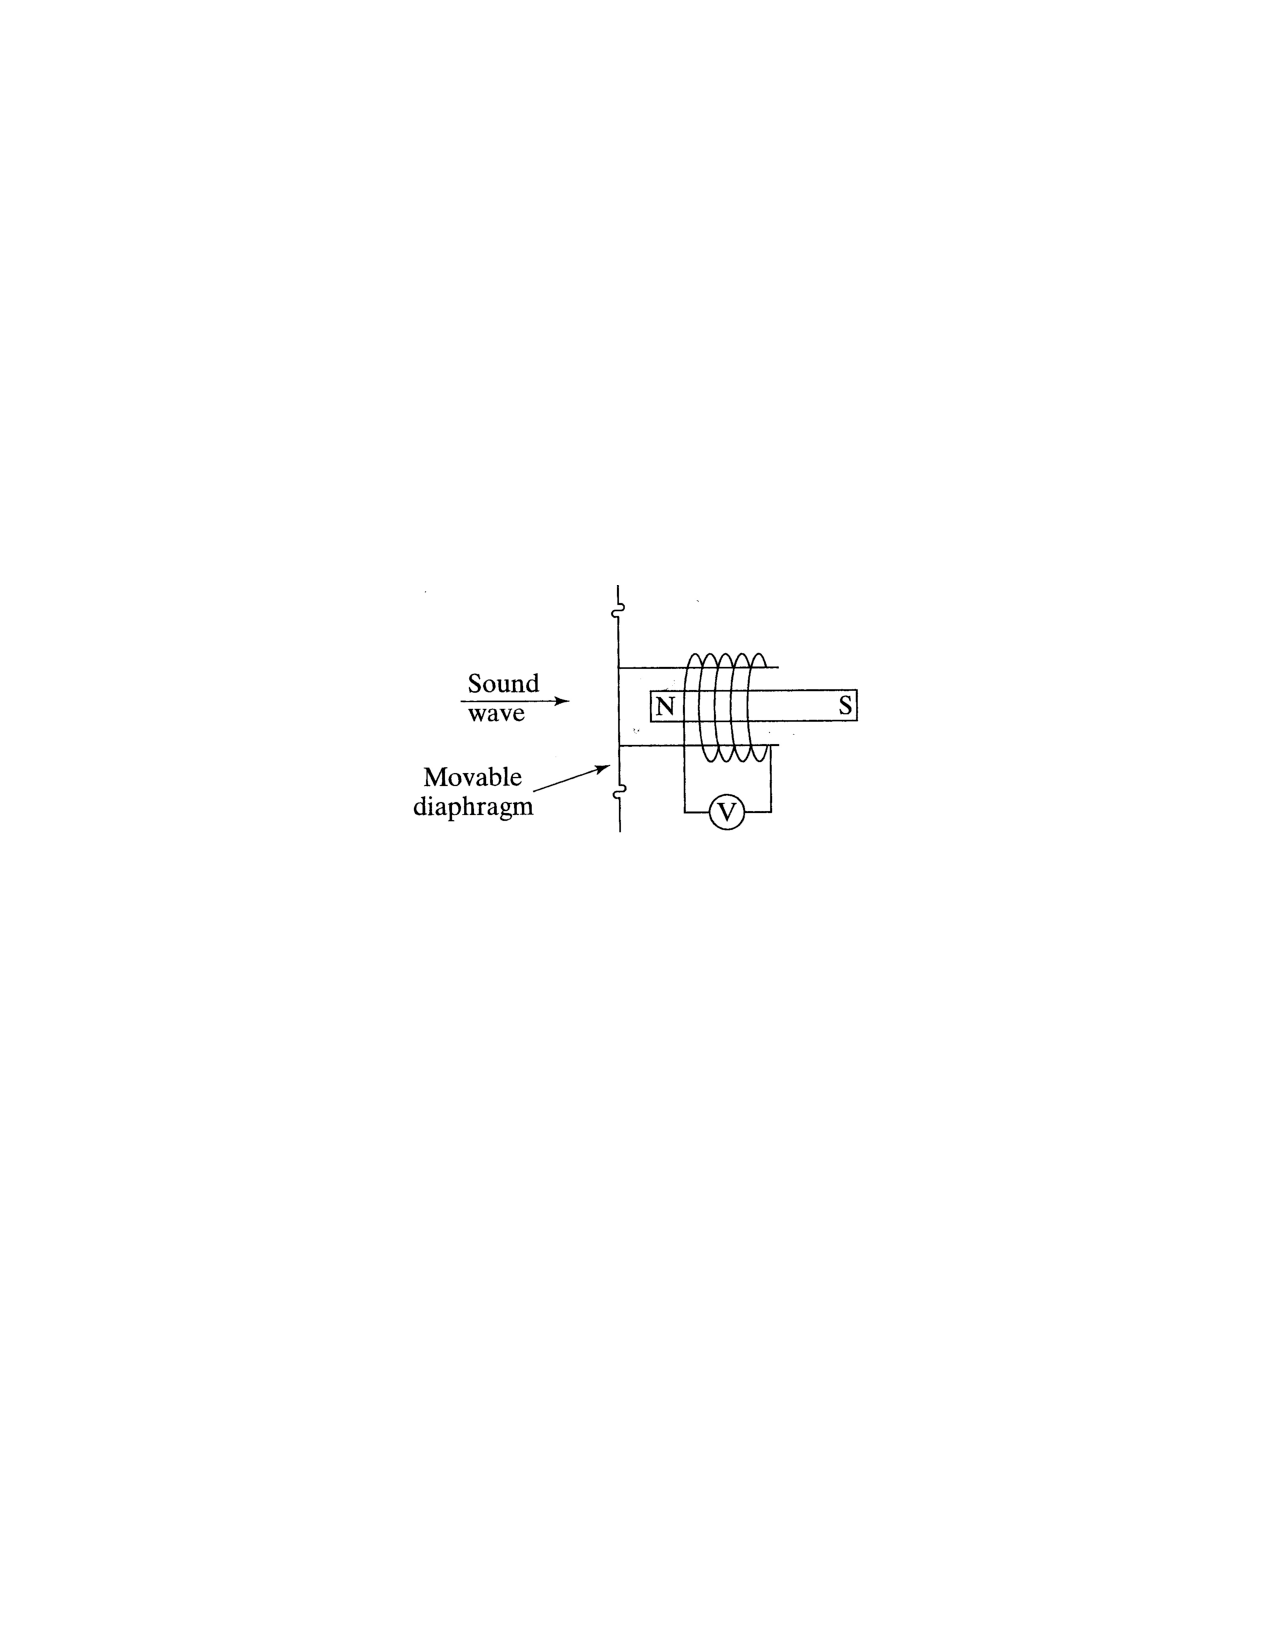
\includegraphics[width=0.5\textwidth]{microphone}
\caption{Schematic diagram of a dynamics microphone.
The pressure deviation associated with a sound wave
pushes back and forth on the diaphragm of the microphone.
A coil of wire, which is attached to the diaphragm, thus
moves in the presence of a magnetic field.
The changing magnetic flux through the coil induces a voltage $V$ in
the coil which follows the fluctuations of the sound wave.
(Figure from ``Physics of Sound," by Berg and Stork.)} 
\label{f:microphone}
\end{center}
\end{figure}
%
%
\begin{figure}[htbp]
\begin{center}
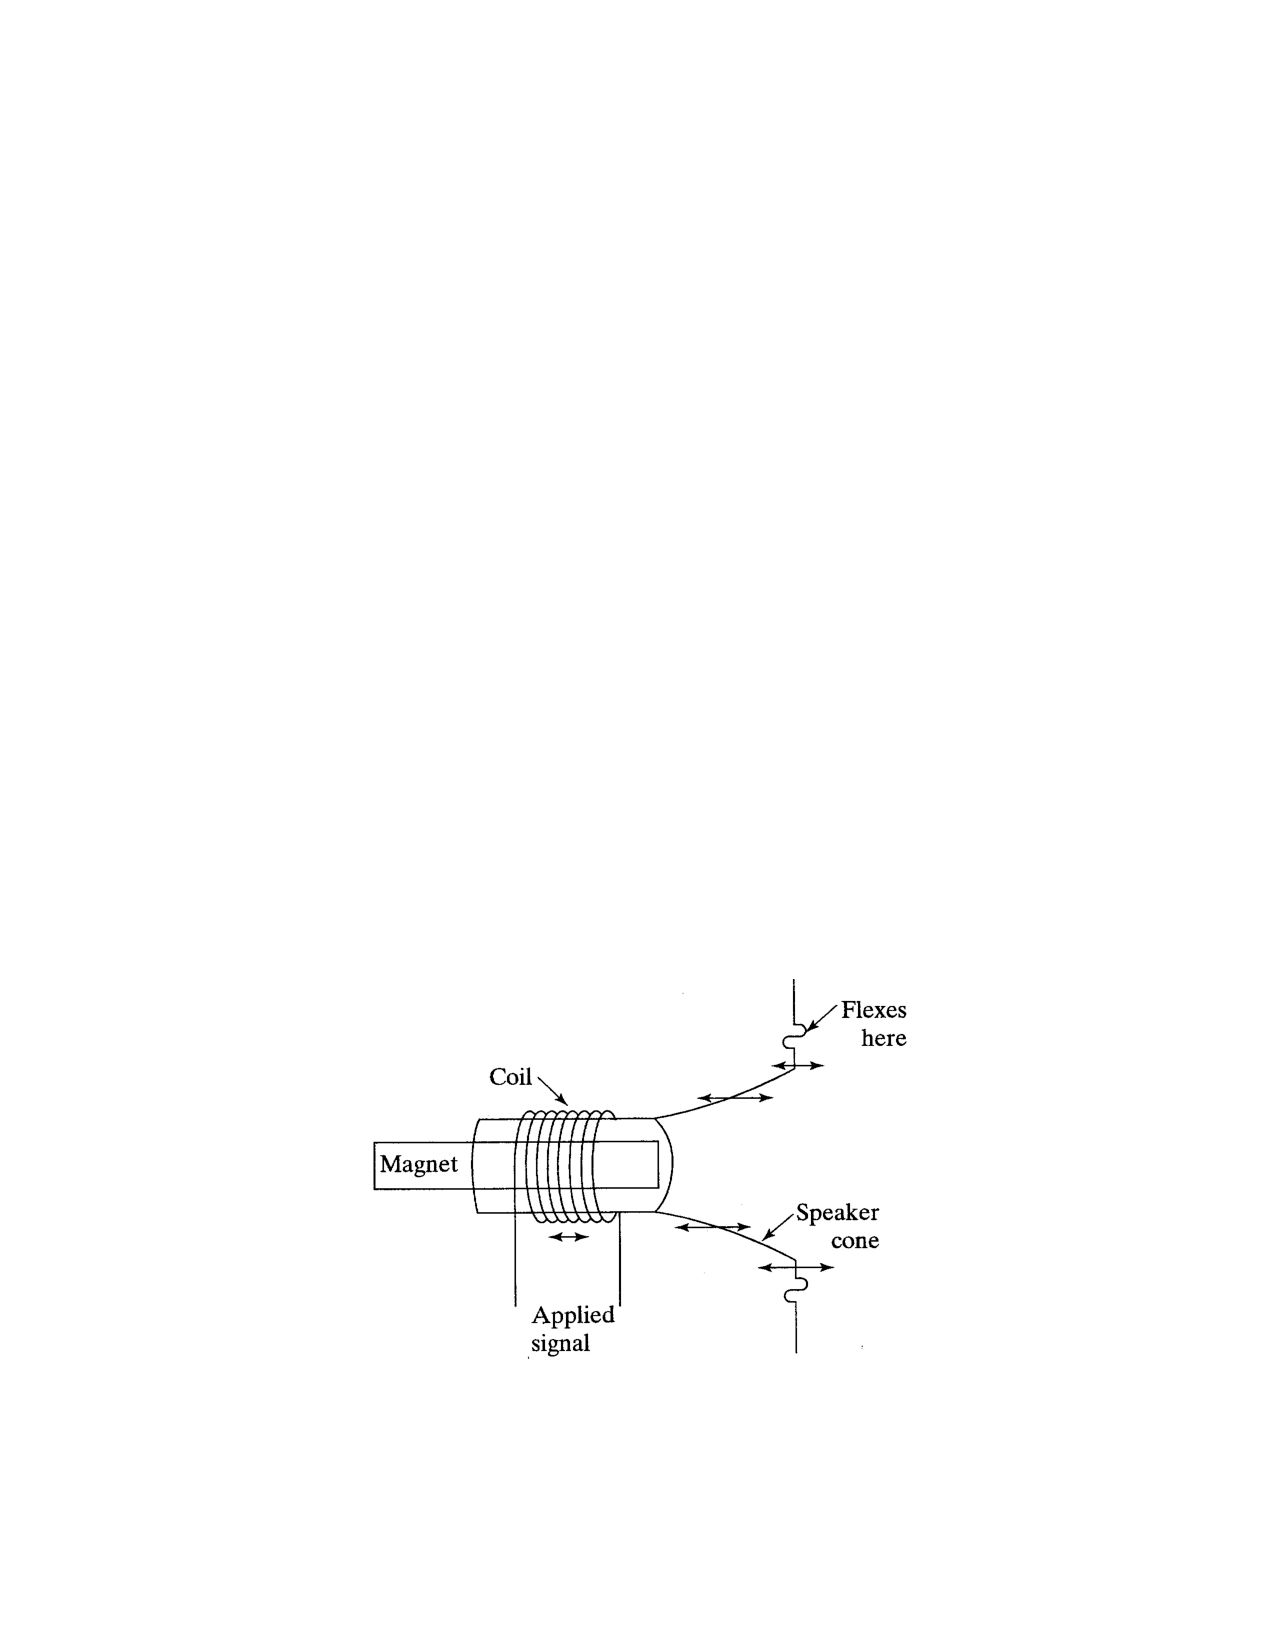
\includegraphics[width=0.5\textwidth]{loudspeaker}
\caption{An electrical signal applied to the coil 
creates a magnetic field that interacts with that of the
permanent magnetic.
The speaker cone, which is attached to the coil, 
moves back-and-forth in repsonse to this interaction,
thus producing a sound wave. 
(Figure from ``Physics of Sound," by Berg and Stork.)} 
\label{f:loudspeaker}
\end{center}
\end{figure}
%
%
\begin{figure}[htbp]
\begin{center}
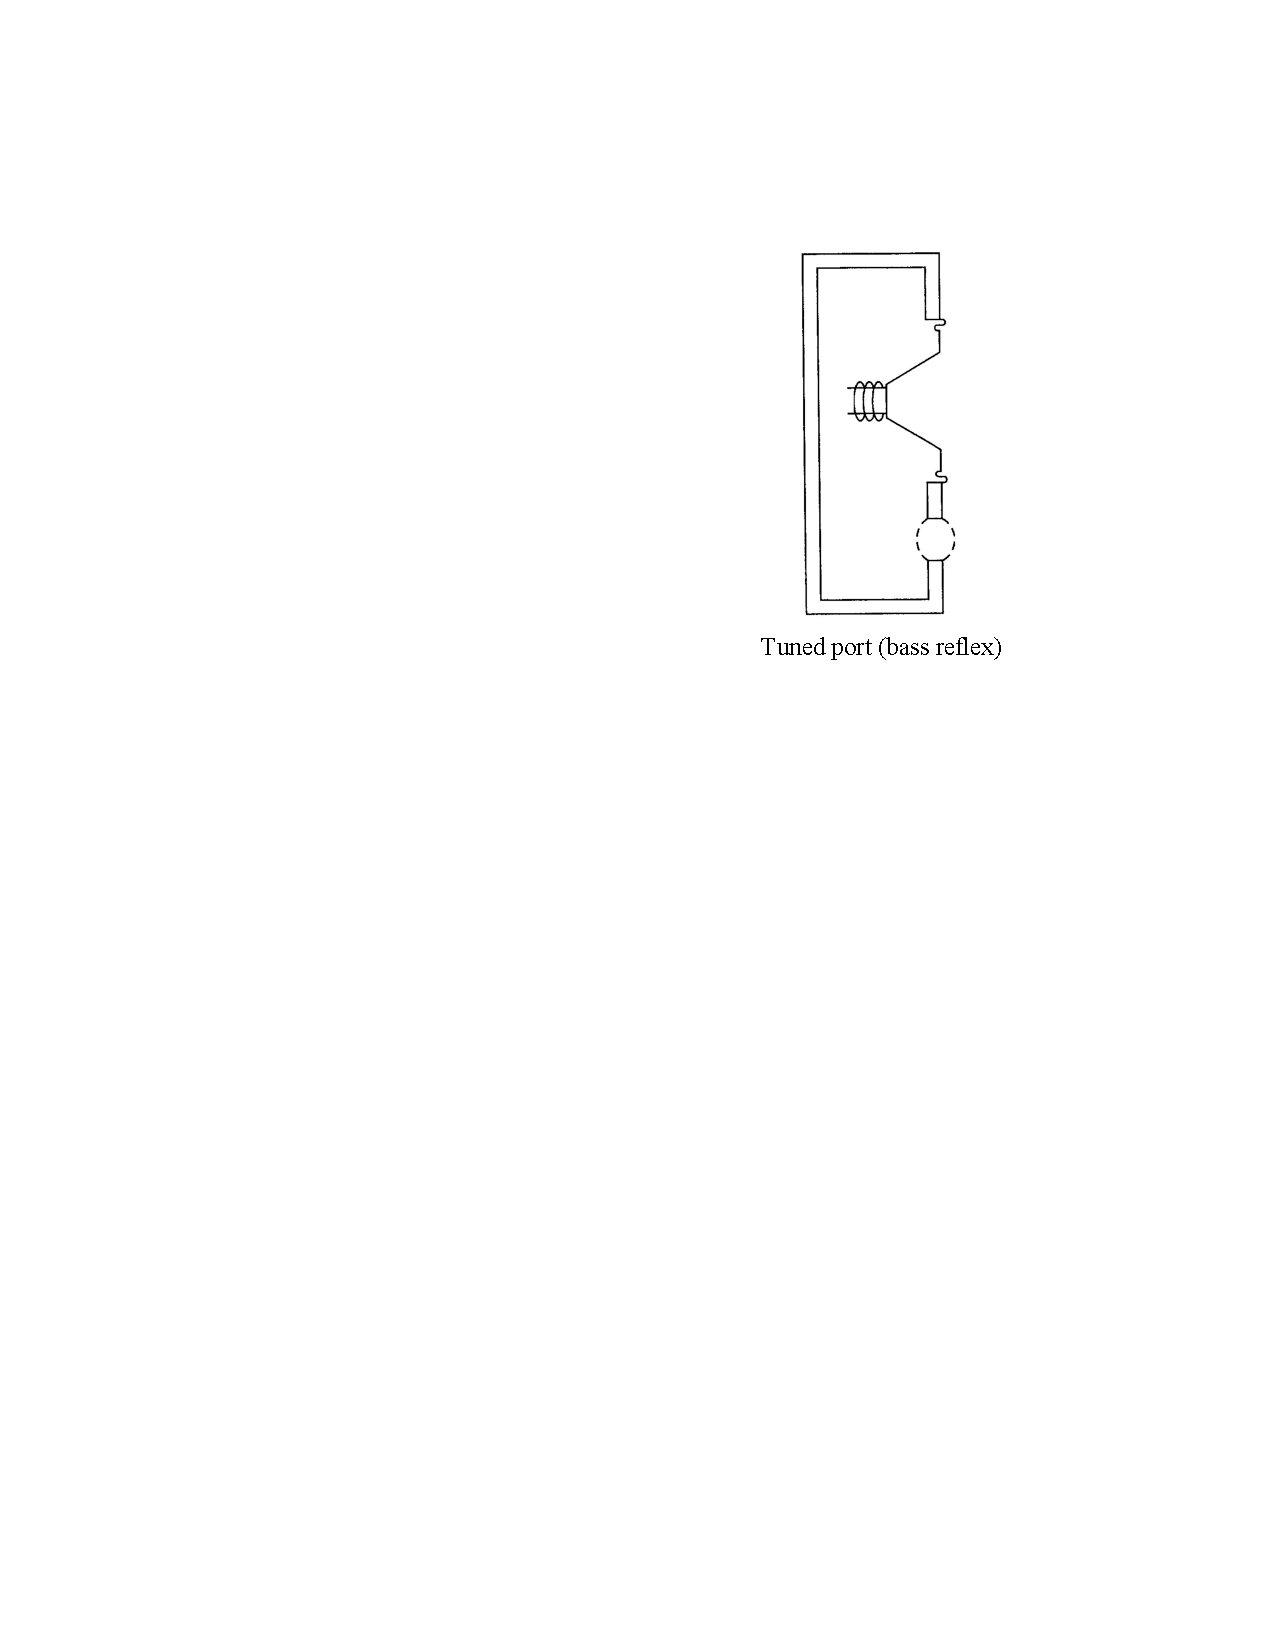
\includegraphics[height=0.4\textwidth]{loudspeaker_tunedport}
\hspace{0.2in}
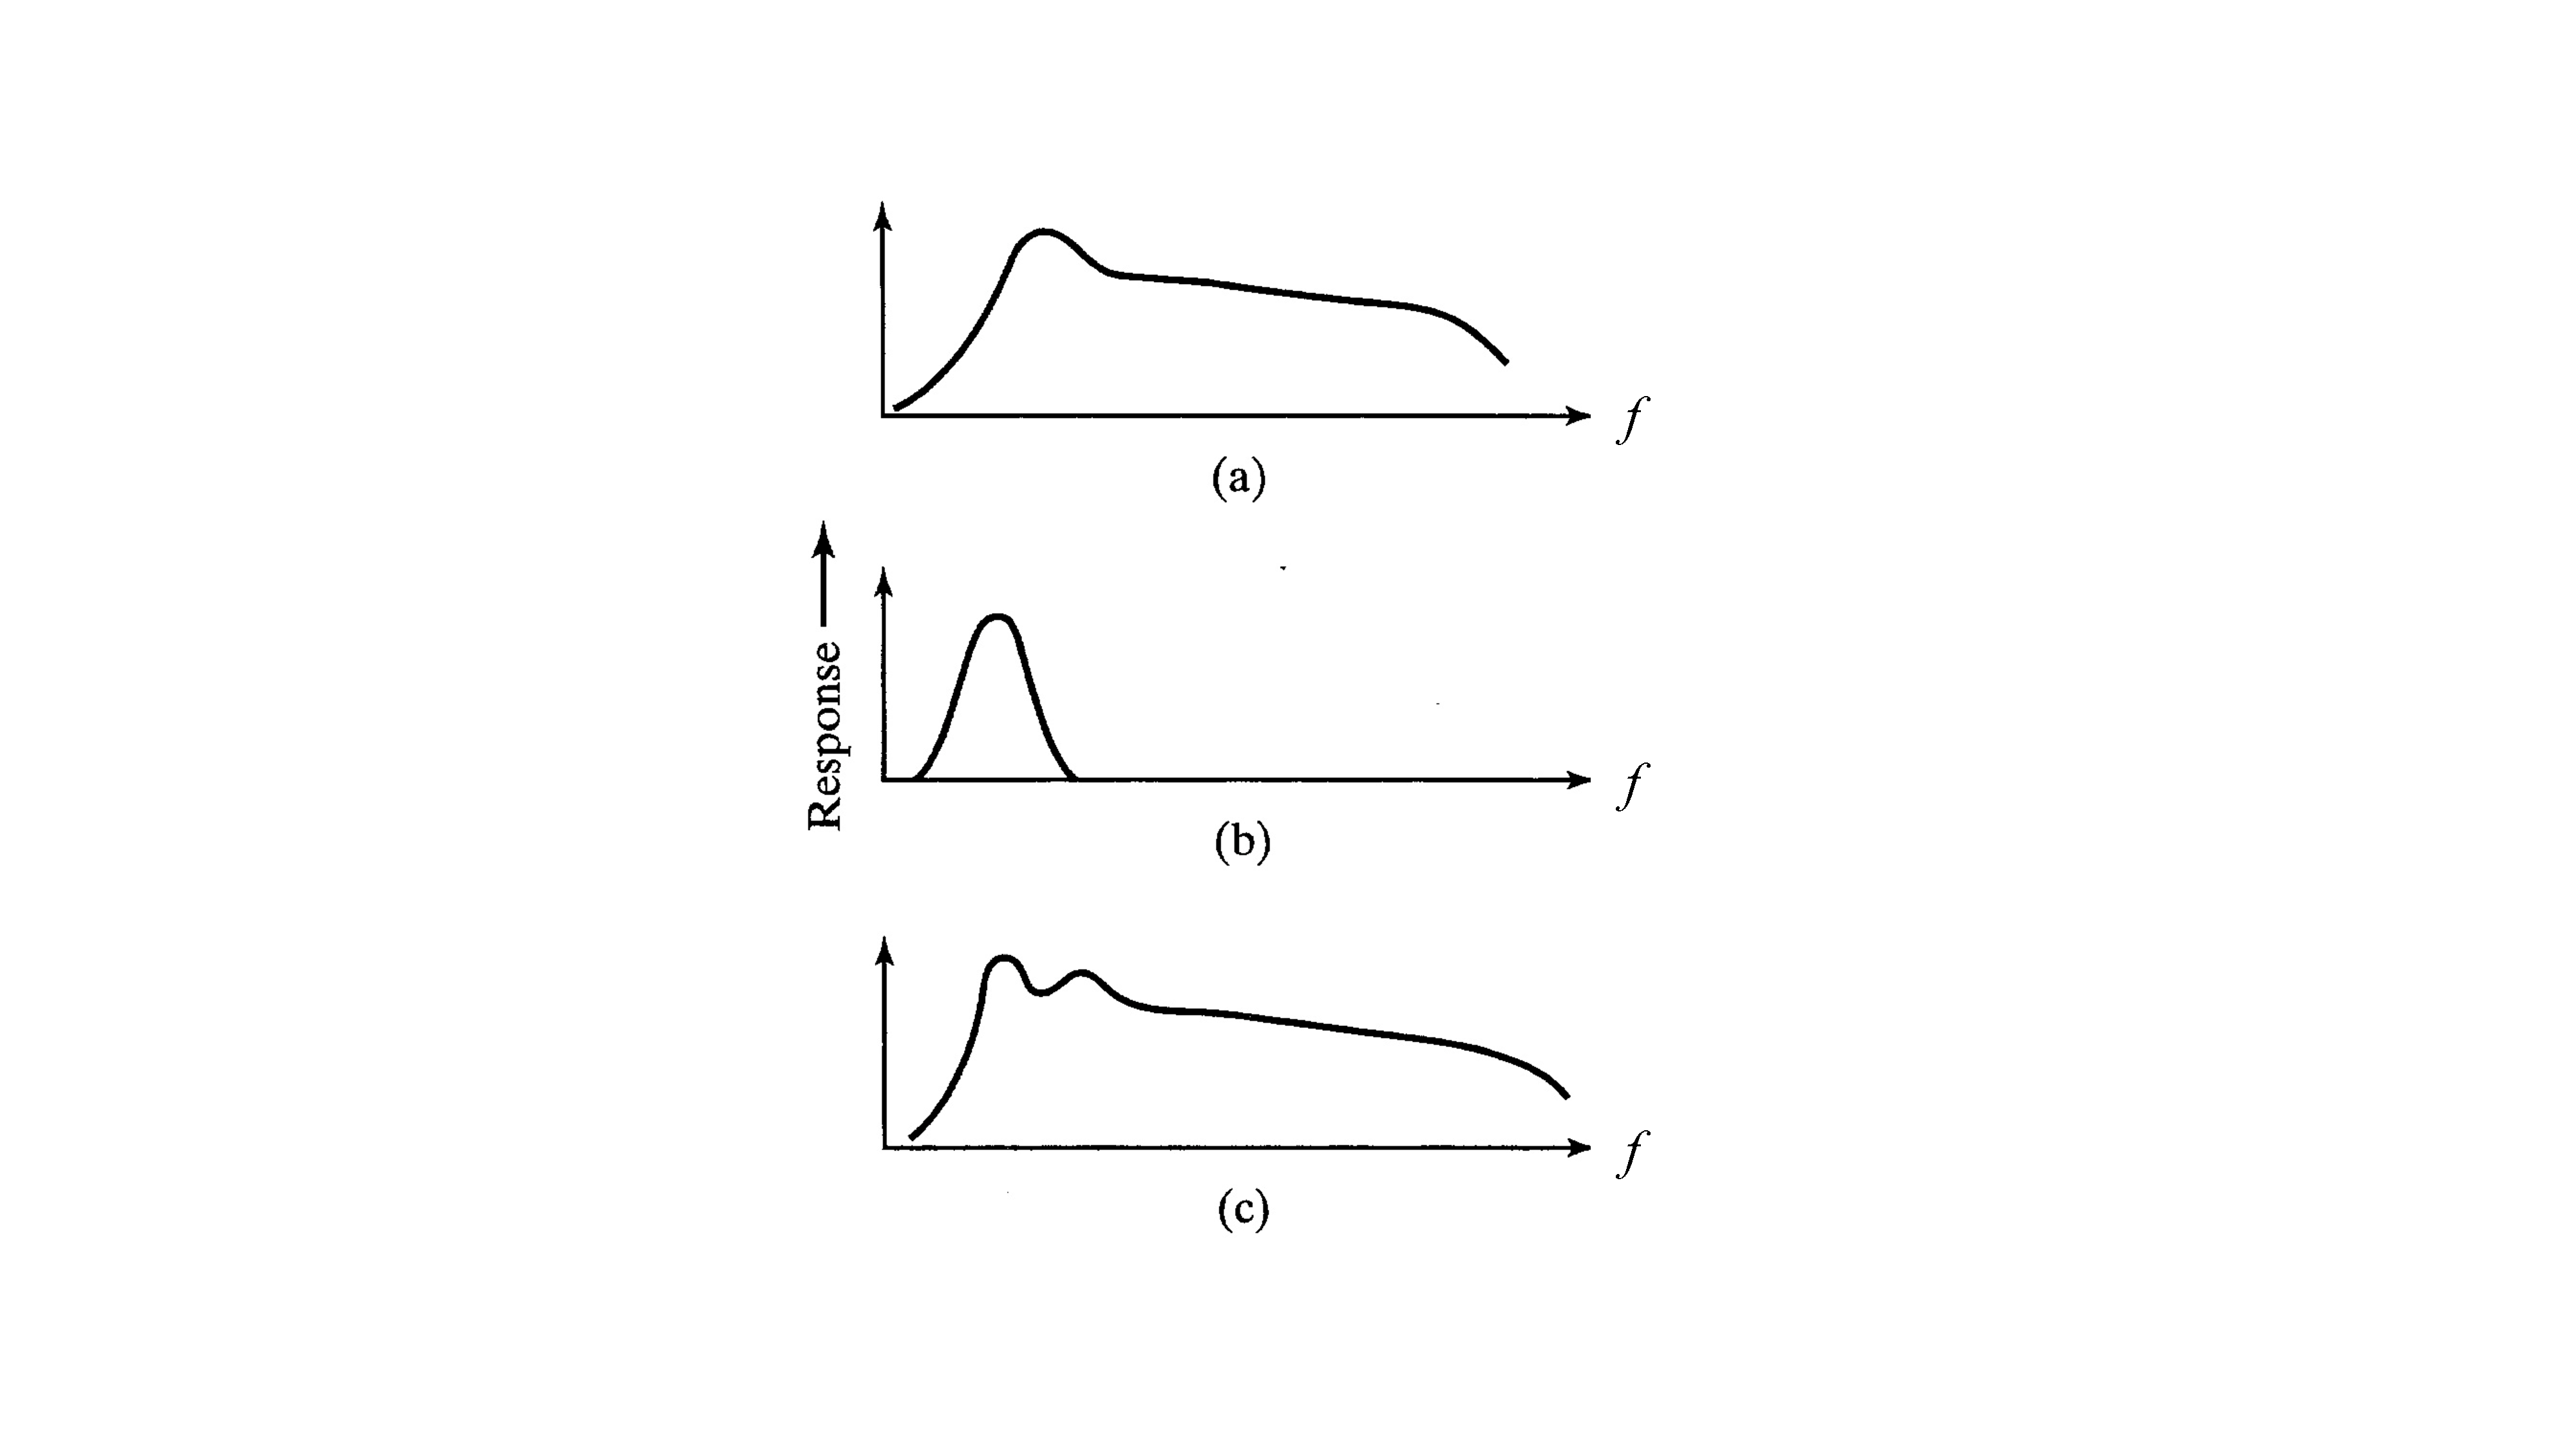
\includegraphics[height=0.4\textwidth]{loudspeaker_tunedport_response}
\caption{Acoustic-suspension and tuned-port loudspeakers (left, middle); 
frequency response curves (right).
(a) Frequency repsonse for an acoustic-suspension loudspeaker.
(b) Frequency response of an empty box with a hole (tuned port), 
which acts like a Helmholtz resonator.
(c) Combined frequency response for a tuned-port loudspeaker.
(Figures from ``Physics of Sound," by Berg and Stork.)} 
\label{f:loudspeaker_tunedport}
\end{center}
\end{figure}
%

